\documentclass{beamer}
\usetheme{Warsaw}
\usepackage{amsmath,amsthm, bm, tikz,qtree}
\usetikzlibrary{arrows,positioning,shapes,fit,calc}
\title{Probabilistic Forecast Reconciliation}
\date{June 20, 2018}
\author[GPAH]{Puwasala Gamakumara, Anastasios Panagiotelis, George Athanasopoulos and Rob Hyndman}
\begin{document}
  \begin{frame}
    \maketitle
  \end{frame}
  \section{Concepts}
  \begin{frame}{Hierarchical and Grouped Time Series}
  	\begin{itemize}
  	  \item Collections of Time Series often characterised by aggregation constraints
  	  \begin{itemize}
  	    \item Cross-Sectionally
  		\item Temporally
  	  \end{itemize}
      \item {\bf Coherent} forecasts respect such constraints. 
      \item Independently produced forecasts are generally incoherent.
  \end{itemize}
\begin{figure}
	\begin{center}
		\leaf{AA} \leaf{AB} 
		\branch{2}{A}
		\leaf{BA} \leaf{BB}
		\branch{2}{B}
		\branch{2}{Tot}
		\qobitree
	\end{center}
\end{figure}
\end{frame}  
  \begin{frame}{Forecast Reconciliation}
  	\begin{itemize}
  	  \item Forecast reconciliation involves
  	  \begin{enumerate}
  	  	\item Producing incoherent {\bf base} forecasts for all series in an $n\times 1$ vector $\hat{\bm y}$
        \item Adjusting base forecasts to obtain {\bf reconciled} forecasts in an $n\times 1$ vector $\tilde{\bm y}$
  	  \end{enumerate} 
      \item Why do we care?
        \begin{enumerate}
        	\item Aligned decision making.
        	\item Improved forecast accuracy
        \end{enumerate}
  	\end{itemize}
  \end{frame}
  \begin{frame}{Reconciliation in two steps}
  	\begin{itemize}
  		\item Many reconciliation methods involve two steps
  		\begin{enumerate}
  			\item Pre-multiply $\hat{\bm y}$ by a $m\times n$ matrix $\bm G$ to obtain {\bf bottom} level series ${\bm b}={\bm G}{\hat{\bm y}}$ 
  			\item Pre-multiply ${\bm b}$ by a $n\times m$ matrix $\bm S$ to obtain ${\tilde{\bm y}}$, i.e. $\tilde{\bm y}={\bm S}{{\bm b}}$
  		\end{enumerate}
  	    \item The matrix ${\bm S}$ defines the aggregation constraints, e.g.
  	    \begin{equation*}
  	    {\bm S}=\begin{pmatrix} 1 &1 &1 &1 \\1 &1 &0 &0 \\0 &0 &1 &1 \\ &{\bm I_{4\times 4}}
  	    \end{pmatrix}
  	    \end{equation*}
  	    \item Choices of ${\bm G}$ defines reconciliation method, e.g. OLS: ${\bm G}=\left(\bm{S}'\bm{S}\right)^{-1}{\bm S'}$ and Bottom Up: ${\bm G}=\left(\bm{0}_{m\times n-m}~\bm{I}_{m\times m}\right)$ 
    \end{itemize}
  \end{frame}
  \begin{frame}{Geometry}
  	\vspace{-2.3cm}
  	\centering
  	% Created by tikzDevice version 0.12 on 2019-08-21 19:50:39
% !TEX encoding = UTF-8 Unicode
\begin{tikzpicture}[x=1pt,y=1pt]
\definecolor{fillColor}{RGB}{255,255,255}
\path[use as bounding box,fill=fillColor,fill opacity=0.00] (0,0) rectangle (289.08,289.08);
\begin{scope}
\path[clip] ( 49.20, 61.20) rectangle (263.88,239.88);
\definecolor{drawColor}{RGB}{0,0,0}

\path[draw=drawColor,line width= 0.4pt,line join=round,line cap=round] ( 87.60, 49.44) --
	( 87.60,196.50);

\path[draw=drawColor,line width= 0.4pt,line join=round,line cap=round] ( 50.84, 86.20) --
	(197.90, 86.20);

\path[draw=drawColor,line width= 1.2pt,line join=round,line cap=round] ( 87.60, 86.20) -- (216.28,150.54);

\path[draw=drawColor,line width= 1.2pt,line join=round,line cap=round] (206.33,135.46) --
	(216.28,150.54) --
	(198.25,151.62);

\node[text=drawColor,anchor=base west,inner sep=0pt, outer sep=0pt, scale=  1.00] at (222.28,148.24) {{\large $\mathfrak{s}$}};
\definecolor{drawColor}{RGB}{0,0,255}
\definecolor{fillColor}{RGB}{0,0,255}

\path[draw=drawColor,line width= 0.4pt,line join=round,line cap=round,fill=fillColor] (142.75,196.50) circle (  3.00);
\definecolor{drawColor}{RGB}{0,0,0}

\node[text=drawColor,anchor=base,inner sep=0pt, outer sep=0pt, scale=  1.00] at (142.75,214.50) {{\large $\color{blue}{\hat{\bm{y}}}$}};
\definecolor{drawColor}{RGB}{255,0,0}
\definecolor{fillColor}{RGB}{255,0,0}

\path[draw=drawColor,line width= 0.4pt,line join=round,line cap=round,fill=fillColor] (175.84,130.32) circle (  3.00);
\definecolor{drawColor}{RGB}{0,0,0}

\node[text=drawColor,anchor=base,inner sep=0pt, outer sep=0pt, scale=  1.00] at (175.84,106.58) {{\large $\color{red}{\tilde{\bm{y}}}$}};
\definecolor{drawColor}{RGB}{0,0,255}

\path[draw=drawColor,line width= 0.4pt,line join=round,line cap=round] (142.75,196.50) -- (175.84,130.32);

\path[draw=drawColor,line width= 0.4pt,line join=round,line cap=round] (160.76,140.27) --
	(175.84,130.32) --
	(176.92,148.35);
\definecolor{drawColor}{RGB}{0,0,0}

\path[draw=drawColor,line width= 0.4pt,dash pattern=on 4pt off 4pt ,line join=round,line cap=round] (142.75,196.50) -- (119.12,101.96);
\definecolor{fillColor}{RGB}{0,0,0}

\path[draw=drawColor,line width= 0.4pt,line join=round,line cap=round,fill=fillColor] (119.12,101.96) circle (  3.00);

\node[text=drawColor,anchor=base,inner sep=0pt, outer sep=0pt, scale=  1.00] at (119.12, 78.22) {{\large $\color{black}{{\bm{y}}}$}};
\end{scope}
\end{tikzpicture}

  \end{frame}
  \begin{frame}{Geometry: Oblique Projection}
  	\vspace{-0.9cm}
  	\centering
  	% Created by tikzDevice version 0.11 on 2018-04-20 18:57:37
% !TEX encoding = UTF-8 Unicode
\begin{tikzpicture}[x=1pt,y=1pt]
\definecolor{fillColor}{RGB}{255,255,255}
\path[use as bounding box,fill=fillColor,fill opacity=0.00] (0,0) rectangle (505.89,361.35);
\begin{scope}
\path[clip] ( 49.20, 61.20) rectangle (480.69,312.15);
\definecolor{drawColor}{RGB}{0,0,0}

\path[draw=drawColor,line width= 0.4pt,line join=round,line cap=round] ( 88.68, 49.37) --
	( 88.68,302.86);

\path[draw=drawColor,line width= 0.4pt,line join=round,line cap=round] (  0.00, 91.62) --
	(505.89, 91.62);

\path[draw=drawColor,line width= 1.2pt,line join=round,line cap=round] ( 88.68, 91.62) -- (417.71,165.55);

\path[draw=drawColor,line width= 1.2pt,line join=round,line cap=round] (404.42,153.31) --
	(417.71,165.55) --
	(400.46,170.93);

\node[text=drawColor,anchor=base west,inner sep=0pt, outer sep=0pt, scale=  1.00] at (423.71,163.26) {{\Large ${\bm S}$}};

\node[text=drawColor,anchor=base,inner sep=0pt, outer sep=0pt, scale=  1.00] at (276.70,112.53) {{\huge $\mathfrak{s}$}};

\path[draw=drawColor,line width= 1.2pt,line join=round,line cap=round] ( 88.68, 91.62) -- (182.69,260.61);

\path[draw=drawColor,line width= 1.2pt,line join=round,line cap=round] (182.98,242.54) --
	(182.69,260.61) --
	(167.19,251.33);

\node[text=drawColor,anchor=base,inner sep=0pt, outer sep=0pt, scale=  1.00] at (182.69,266.61) {{\Large ${\bm R}$}};

\path[draw=drawColor,line width= 0.4pt,dash pattern=on 4pt off 4pt ,line join=round,line cap=round] (108.22,  0.00) --
	(276.70,302.86);
\definecolor{drawColor}{RGB}{0,0,255}
\definecolor{fillColor}{RGB}{0,0,255}

\path[draw=drawColor,line width= 0.4pt,line join=round,line cap=round,fill=fillColor] (229.69,218.36) circle (  3.00);
\definecolor{drawColor}{RGB}{0,0,0}

\node[text=drawColor,anchor=base,inner sep=0pt, outer sep=0pt, scale=  1.00] at (229.69,236.36) {{\huge $\color{blue}{\hat{\bm{y}}}$}};

\node[text=drawColor,anchor=base west,inner sep=0pt, outer sep=0pt, scale=  1.00] at (212.19,173.82) {{\huge ${\color{blue} s\circ g}$}};
\definecolor{drawColor}{RGB}{255,0,0}
\definecolor{fillColor}{RGB}{255,0,0}

\path[draw=drawColor,line width= 0.4pt,line join=round,line cap=round,fill=fillColor] (169.26,109.72) circle (  3.00);
\definecolor{drawColor}{RGB}{0,0,0}

\node[text=drawColor,anchor=base,inner sep=0pt, outer sep=0pt, scale=  1.00] at (169.26, 85.99) {{\huge $\color{red}{\tilde{\bm{y}}}$}};
\definecolor{drawColor}{RGB}{0,0,255}

\path[draw=drawColor,line width= 0.4pt,line join=round,line cap=round] (229.69,218.36) -- (169.26,109.72);

\path[draw=drawColor,line width= 0.4pt,line join=round,line cap=round] (168.97,127.79) --
	(169.26,109.72) --
	(184.76,119.01);
\end{scope}
\end{tikzpicture}

  \end{frame}
  \section{Probabilistic Reconciliation}
  \begin{frame}{Coherent Subspace}
  	\begin{definition} 
  		The {\bf coherent subspace} is the linear subspace spanned by the columns of ${\bm S}$, i.e. $\mathfrak{s}=\mbox{sp}({\bm S})$
  	\end{definition}
    Instead of using bottom-level series a different combination of $m$ {\bf basis series} could be used (e.g. top and $m-1$ bottom).  Although ${\bm S}$ would be different $\mathfrak{s}$ would be the same.
  \end{frame}
  \begin{frame}{Coherent Probabilistic Forecast}
    Let $(\mathbb{R}^m,\mathcal{F}_{\mathbb{R}^m},\nu)$ and $(\mathfrak{s},\mathcal{F}_{\mathfrak{s}},\mu)$ be probability triples on $m$-dimensional space and the coherent subspace respectively.
    \begin{definition}
      The probability measure $\nu_{\mathfrak{s}}$ is coherent if
      \begin{equation*}
      \nu(\mathcal{B})=\mu(s(\mathcal{B}))\quad\forall\mathcal{B}\in \mathcal{F}_{\mathcal{R}_m}
      \end{equation*} 
    \end{definition}
    where $s(\mathcal{B})$ is the image of $\mathcal{B}$ under premultiplication by ${\bm S}$
  \end{frame}
  \begin{frame}{Reconciled Probabilistic Forecast}
  	Let $g:\mathbb{R}^n\rightarrow\mathbb{R}^m$ be a linear map.  Then 
  	\begin{definition}
  	The probability triple $\left(\mathfrak{s},\mathcal{F}_{\mathfrak{s}},\tilde{\nu}\right)$ is the reconciles the probability triple $\left(\mathbb{R}^n,\mathcal{F}_{\mathbb{R}^n},\hat{\nu}\right)$ with with respect to $g$ iff
  	\begin{equation*}
  	\tilde{\nu}(s(\mathcal{B}))=\nu(\mathcal{B})=\hat{\nu}(g^{-1}(\mathcal{B}))\quad\forall \mathcal{B}\in\mathcal{F}_{\mathcal{R}_m}
  	\end{equation*}
  	\end{definition}
    where $g^{-1}$ is the pre-image of $g$.
  \end{frame}
  \begin{frame}{Geometry}
  	\centering
  	% Created by tikzDevice version 0.11 on 2018-04-20 18:17:41
% !TEX encoding = UTF-8 Unicode
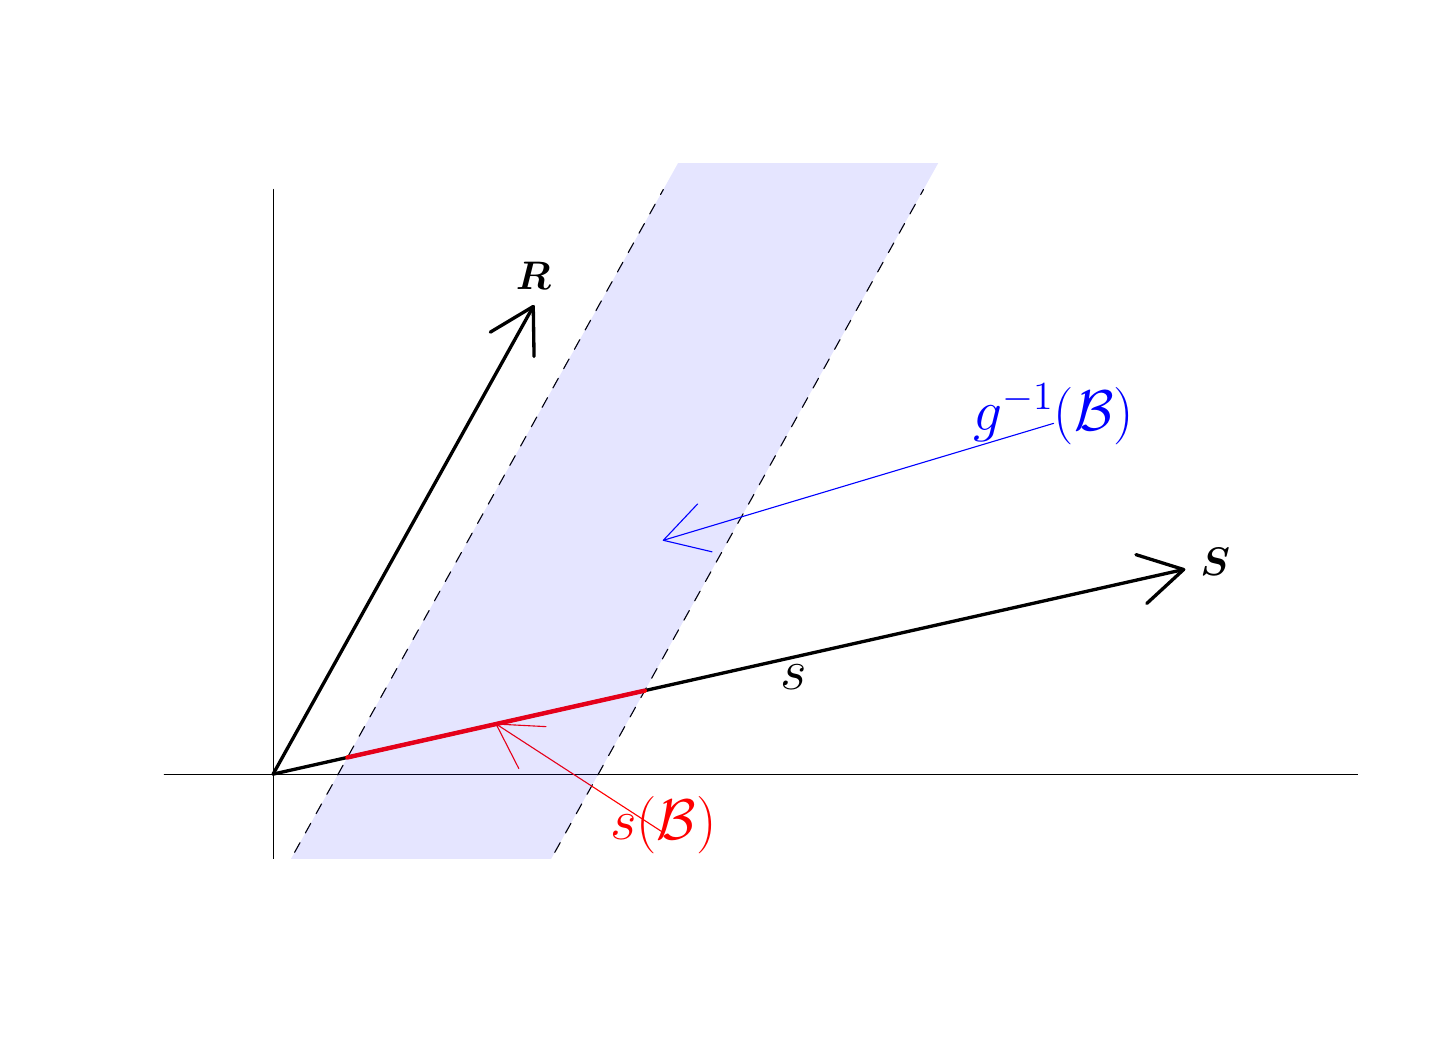
\begin{tikzpicture}[x=1pt,y=1pt]
\definecolor{fillColor}{RGB}{255,255,255}
\path[use as bounding box,fill=fillColor,fill opacity=0.00] (0,0) rectangle (505.89,361.35);
\begin{scope}
\path[clip] ( 49.20, 61.20) rectangle (480.69,312.15);
\definecolor{drawColor}{RGB}{0,0,0}

\path[draw=drawColor,line width= 0.4pt,line join=round,line cap=round] ( 88.68, 49.37) --
	( 88.68,302.86);

\path[draw=drawColor,line width= 0.4pt,line join=round,line cap=round] (  0.00, 91.62) --
	(505.89, 91.62);

\path[draw=drawColor,line width= 1.2pt,line join=round,line cap=round] ( 88.68, 91.62) -- (417.71,165.55);

\path[draw=drawColor,line width= 1.2pt,line join=round,line cap=round] (404.42,153.31) --
	(417.71,165.55) --
	(400.46,170.93);

\node[text=drawColor,anchor=base west,inner sep=0pt, outer sep=0pt, scale=  1.00] at (423.71,163.26) {{\Large ${\bm S}$}};

\node[text=drawColor,anchor=base,inner sep=0pt, outer sep=0pt, scale=  1.00] at (276.70,122.13) {{\huge $\mathfrak{s}$}};

\path[draw=drawColor,line width= 1.2pt,line join=round,line cap=round] ( 88.68, 91.62) -- (182.69,260.61);

\path[draw=drawColor,line width= 1.2pt,line join=round,line cap=round] (182.98,242.54) --
	(182.69,260.61) --
	(167.19,251.33);

\node[text=drawColor,anchor=base,inner sep=0pt, outer sep=0pt, scale=  1.00] at (182.69,266.61) {{\Large ${\bm R}$}};

\path[draw=drawColor,line width= 0.4pt,dash pattern=on 4pt off 4pt ,line join=round,line cap=round] ( 88.68, 49.37) --
	(229.69,302.86);

\path[draw=drawColor,line width= 0.4pt,dash pattern=on 4pt off 4pt ,line join=round,line cap=round] (182.69, 49.37) --
	(323.70,302.86);
\definecolor{drawColor}{RGB}{255,0,0}

\path[draw=drawColor,line width= 1.6pt,line join=round,line cap=round] (115.54, 97.65) --
	(222.98,121.79);
\definecolor{drawColor}{RGB}{0,0,0}

\node[text=drawColor,anchor=base,inner sep=0pt, outer sep=0pt, scale=  1.00] at (229.69, 68.00) {{\huge $\color{red}{s(\mathcal{B})}$}};
\definecolor{drawColor}{RGB}{255,0,0}

\path[draw=drawColor,line width= 0.4pt,line join=round,line cap=round] (229.69, 70.49) -- (169.26,109.72);

\path[draw=drawColor,line width= 0.4pt,line join=round,line cap=round] (187.30,108.78) --
	(169.26,109.72) --
	(177.47, 93.63);
\definecolor{fillColor}{RGB}{0,0,255}

\path[fill=fillColor,fill opacity=0.10] ( 65.18,  7.12) --
	(159.19,  7.12) --
	(347.20,345.10) --
	(253.19,345.10) --
	cycle;
\definecolor{drawColor}{RGB}{0,0,255}

\node[text=drawColor,anchor=base,inner sep=0pt, outer sep=0pt, scale=  1.00] at (370.70,215.86) {{\huge $\color{blue}{g^{-1}(\mathcal{B}})$}};

\path[draw=drawColor,line width= 0.4pt,line join=round,line cap=round] (370.70,218.36) -- (229.69,176.11);

\path[draw=drawColor,line width= 0.4pt,line join=round,line cap=round] (242.09,189.26) --
	(229.69,176.11) --
	(247.27,171.95);
\end{scope}
\end{tikzpicture}

  \end{frame}
  \begin{frame}{Analytically}
  	If we have an unreconciled density the reconciled density can be obtained by linear transformations and marginalisation.
  	\begin{align*}
  	\mbox{Pr}(\tilde{\bm{b}}\in s(\mathcal{B}))&=\mbox{Pr}(\hat{\bm{y}}\in g^{-1}(\mathcal{B}))\\
  	&=\int\limits_{g^{-1}(\mathcal{B})}f(\hat{\bm{y}})d\hat{\bm{y}}\\
  	&=\int\limits_{\mathcal{B}}\int f(\bm{S}\tilde{\bm{b}}+\bm{R}\tilde{\bm{a}})|\left(\bm{S}~\bm{R}\right)|d\tilde{\bm{a}}d\tilde{\bm{b}}
  	\end{align*}
  \end{frame}
  \begin{frame}{Elliptical distributions}
  	Let the unreconciled density be elliptical with location  $\hat{\bm{\mu}}$ and scale $\hat{\bm{\Sigma}}$ and let the true predictive density be elliptical with location  ${\bm{\mu}}$ and scale ${\bm{S}}{\bm{\Omega}}{\bm{S}}'$.
  	\begin{theorem}
  		The true predictive distribution can be recovered via linear reconciliation.  The optimal (but infeasible) mapping is $g(\breve{\bm y})={\bm G}_{opt}\breve{\bm y}+{\bm d}_{opt}$ where $\bm{G}_{opt}={\bm\Omega}^{1/2}{\bm\hat{\Sigma}}^{-1/2}$ and ${\bm d}_{opt}={\bm S}{\bm G}_{opt}\left({\bm \mu}-\hat{\bm \mu}\right)$.
  	\end{theorem}
    This follows from the closure property of elliptical distributions under affine transformations and marginalisation.
  \end{frame}
  \begin{frame}{With a sample}
  	\begin{itemize}
  		\item Often densities are unavailable but we can simulate a sample from the predictive distribution.
  		\item Suppose $\bm{\hat{y}}^{[1]},\ldots,\bm{\hat{y}}^{[J]}$ is a sample from the unreconciled probabilistic forecast.
  		\item Then setting $\tilde{\bm y}^{[j]}=s\circ g(\hat{\bm y}^{[j]})=\bm{S}\bm{G}\hat{\bm y}^{[j]}$ produces a sample from the reconciled distribution with respect to $g$.
  	\end{itemize}
  \end{frame}
  \section{Scoring}
  \begin{frame}{Univariate v Multivariate Scores}
    Scoring rules can be used to evaluate probabilistic forecasts
    \begin{itemize}
    	\item Univariate
    	\begin{itemize}
    		\item Log Score
    		\item Continuous Rank Probability Score
    	\end{itemize}
    	\item Multivariate
        \begin{itemize}
	      \item Log Score
	      \item Energy Score
        \end{itemize}
    \end{itemize}
    These may be computed using densities or a sample.
  \end{frame}
  \begin{frame}{Approaches}
  	\begin{enumerate}
  		\item Use a summary of all univariate scores.
  		\item Make comparisons on the joint distribution of bottom level series only.
        \item Make comparisons using the full joint distribution
  \end{enumerate}
  There are pitfalls to the third approach.
  \end{frame}
  \begin{frame}{Reconciled v Unreconciled}
	When comparing reconciled and unreconciled probabilistic forecasts on the basis of log score
	\begin{theorem}
		Let $f(\bm{y})$ be the true predictive density (on $\mathfrak{s}$) and $LS$ be the (negatively-oriented) log score.  Then there exists an unreconciled density  $\hat{f}(\bm{y})$ on $\mathbb{R}^n$ such that
		\begin{equation*}
		E_{\bm y}\left[S(\hat{f},\bm{y})\right]<E_{\bm y}\left[S(f,\bm{y})\right]
		\end{equation*}
	\end{theorem}
    The log score is not proper {\bf in this context}.
  \end{frame}
  \begin{frame}{Reconciled v Reconciled}
	\begin{itemize}
		\item For two reconciled probabilistic forecasts log score can be used.
		\item Comparisons can be made on the basis of bottom level series (or any basis series).
		\item By the definition of coherence $\log (f({\bm b}))=\log (f({\bm S}{\bm b}){\bm J})$
		\item The Jacobian does not affect the ordering of log score.
	\end{itemize}
  \end{frame}
  \begin{frame}{Energy  score}
  	\begin{itemize}
  		\item More care must be taken using the energy score.
  		\item Energy score is invariant to orthogonal transformation but not affine transformations.
  		\item Since ${\bm S}$ is not a rotation the ranking of different methods based on the full hierarchy may differ from the ranking based on bottom level series only.
  	\end{itemize}
  \end{frame}
   \begin{frame}{Simulations}
   	\begin{itemize}
   		\item If you want to see tables with numbers look at the paper.
   		\item The main takeaway messages are:
   		    \begin{itemize}
   		    	\item Reconciliation is better than no reconciliation.
   		    	\item Bottom up does not do well.
   		    	\item MinT (an oblique projection) does well.
   		    \end{itemize} 
   	\end{itemize}
   \end{frame}
   \begin{frame}{Looking ahead}
     \begin{itemize}
     	\item The optimal feasible reconciliation method remains an open question even for elliptical distributions.
     	\begin{itemize}
     		\item It is likely to depend on the specific score used.
     	\end{itemize}
        \item Are non-linear reconciliation methods worthwhile?
        \item How should probabilistic reconciliation work for non-elliptical distributions.
        \item Further development of multivariate scoring rules.
     \end{itemize}	
   \end{frame}
\end{document}